% TimeCatch poster — "What's the Catch? Evaluating Temporal Consistency in VLMs"
% A0 portrait, single-column, six story beats.
% Minimal design: white page, hairline separators, typographic hierarchy;
% color appears only in data elements (bars, frame highlights, chart lines)
% plus the KU-crimson title and beat numbers.
\documentclass[a0,portrait]{a0poster}

\usepackage{graphicx}
\usepackage[svgnames]{xcolor}
\usepackage[T1]{fontenc}
% fonts matched to Figure 1: Inter for text, Montserrat for headings
\usepackage{inter}
\renewcommand{\familydefault}{\sfdefault}
\newcommand{\headfamily}{\fontfamily{Montserrat-TLF}\selectfont}
\usepackage{tikz}
\usetikzlibrary{arrows.meta}
\usepackage{pgfplots}
\pgfplotsset{compat=1.18}
\usepackage{amssymb}

% ---------------------------------------------------------------- colors
\definecolor{ku}{RGB}{144,26,30}        % KU crimson: title + beat numbers
\definecolor{hookteal}{RGB}{30,110,90}
\definecolor{neutral}{RGB}{100,106,116}
\definecolor{coral}{RGB}{197,80,62}     % temporal anomaly
\definecolor{grape}{RGB}{94,79,162}     % frame-level anomaly
\definecolor{ink}{RGB}{45,50,56}        % body text / human bars

\parindent=0pt
\pagestyle{empty}
\color{ink}

% ---------------------------------------------------------------- helpers
% beat header: hairline, crimson number, title
\newcommand{\beat}[2]{%
  {\color{ink!22}\hrule height 1pt}
  \vspace{5mm}
  {\huge\bfseries\headfamily {\color{ku}#1}\hspace{6mm}#2\par}
  \vspace{6mm}}

\pgfplotsset{mini/.style={
  width=21cm, height=7.6cm,
  title style={font=\LARGE\bfseries\headfamily, text=ink},
  axis x line*=bottom, axis y line*=left,
  axis line style={line width=1pt, ink!60},
  every tick/.append style={ink!60, line width=1pt},
  tick label style={font=\normalsize, text=ink!80},
  label style={font=\large, text=ink!80},
  legend style={font=\normalsize, draw=none, fill=none},
  ymajorgrids, grid style={ink!12},
  axis on top, clip=false
}}

\begin{document}

% ================================================================ TITLE
\begin{minipage}[b]{0.66\linewidth}
  {\VeryHuge\headfamily \textbf{\textcolor{ku}{What's the Catch?}}}
\end{minipage}
\hfill
\begin{minipage}[b]{0.30\linewidth}
  \raggedleft
  % TimeCatch mark: a four-frame strip with the 3rd/4th frames swapped
  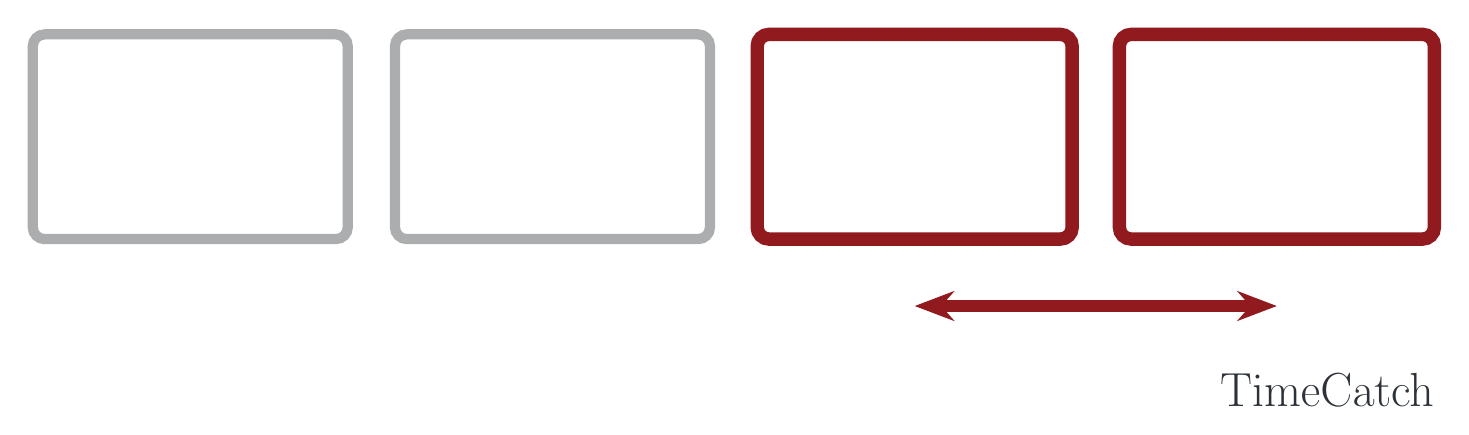
\begin{tikzpicture}[x=1cm,y=1cm]
    \foreach \i in {0,1}{
      \draw[ink!40,line width=1.3mm,rounded corners=1.5mm] (\i*4.6,0) rectangle (\i*4.6+4,2.6);}
    \foreach \i in {2,3}{
      \draw[ku,line width=1.7mm,rounded corners=1.5mm] (\i*4.6,0) rectangle (\i*4.6+4,2.6);}
    \draw[{Stealth[length=5mm]}-{Stealth[length=5mm]},ku,line width=1.5mm]
      (11.2,-0.85) -- (15.8,-0.85);
    \node[anchor=north east,font=\LARGE\bfseries\headfamily,text=ink,inner sep=0]
      at (17.8,-1.7) {TimeCatch};
  \end{tikzpicture}
\end{minipage}\\[8mm]
{\huge\headfamily \textbf{\textcolor{ku}{Evaluating Temporal Consistency in Vision-Language Models}}}\\[7mm]
{\LARGE\itshape Vision-language models can spot a corrupted frame --- but not a reordered one.}
\hfill
{\Large\color{ink!70} Anonymous ACL submission}

\vspace{8mm}

% ================================================================ BEAT 1 — HOOK
\beat{1}{Try it --- can you spot the swap?}
{\Large Four frames from one Olympic dive. \textbf{Two adjacent frames have been swapped.} Which two?}\\[8mm]
\centering
\begin{tikzpicture}[x=1cm,y=1cm]
  \foreach \img/\i in {dive1/0,dive2/1,dive4/2,dive3/3}{
    \node[inner sep=0] at (\i*15.8,0) {\includegraphics[width=15.2cm]{img/\img.jpg}};
    \node[font=\Large\bfseries,text=ink!70] at (\i*15.8,-5.0) {\pgfmathparse{int(\i+1)}\pgfmathresult};}
\end{tikzpicture}\\[7mm]
\raggedright

% ================================================================ BEAT 2 — PROBLEM
\beat{2}{What we test, and why it is hard to measure}
\begin{minipage}[t]{0.31\linewidth}
  \raggedright
  {\Large {\bfseries The question.} Does a VLM connect information \emph{across} frames, or does it only read each frame in isolation?}
\end{minipage}\hfill
\begin{minipage}[t]{0.31\linewidth}
  \raggedright
  {\Large {\bfseries The problem.} Many video benchmarks can be solved from a single frame or from language shortcuts --- a high score does not prove temporal understanding.}
\end{minipage}\hfill
\begin{minipage}[t]{0.31\linewidth}
  \raggedright
  {\Large {\bfseries The stakes.} Driving, robotics, and video understanding depend on recognizing how a scene \emph{evolves}, not just what is in one frame.}
\end{minipage}

\vspace{9mm}

% ================================================================ BEAT 3 — HERO
% Figure 1 from the paper (vector): frame strips, task questions, human-vs-VLM bars
\beat{3}{The catch: models see broken frames, not broken time}
\centering

\includegraphics[width=0.84\linewidth]{img/visual_abstract.pdf}\\[5mm]
{\LARGE\itshape Models detect and localize a corrupted frame reliably. They cannot detect or localize a reordered one. Humans do both near-perfectly.}\\[8mm]
\raggedright

% ================================================================ BEATS 4 + 5
\begin{minipage}[t]{0.34\linewidth}
  \beat{4}{The benchmark}
  \centering
  \begin{tabular}{@{}c@{\hspace{7mm}}c@{}}
    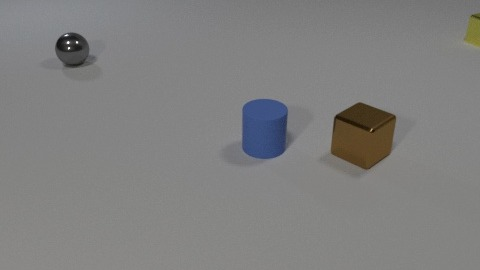
\includegraphics[width=12.8cm]{img/thumb_clevrer.jpg} &
    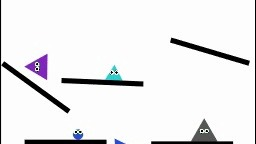
\includegraphics[width=12.8cm]{img/thumb_craft.jpg} \\[2mm]
    {\Large\textbf{CLEVRER} · synthetic} & {\Large\textbf{CRAFT} · synthetic} \\[1mm]
    {\large\color{ink!70} 4{,}997 seq · avg 7.5 frames} & {\large\color{ink!70} 858 seq · avg 6.9 frames} \\[7mm]
    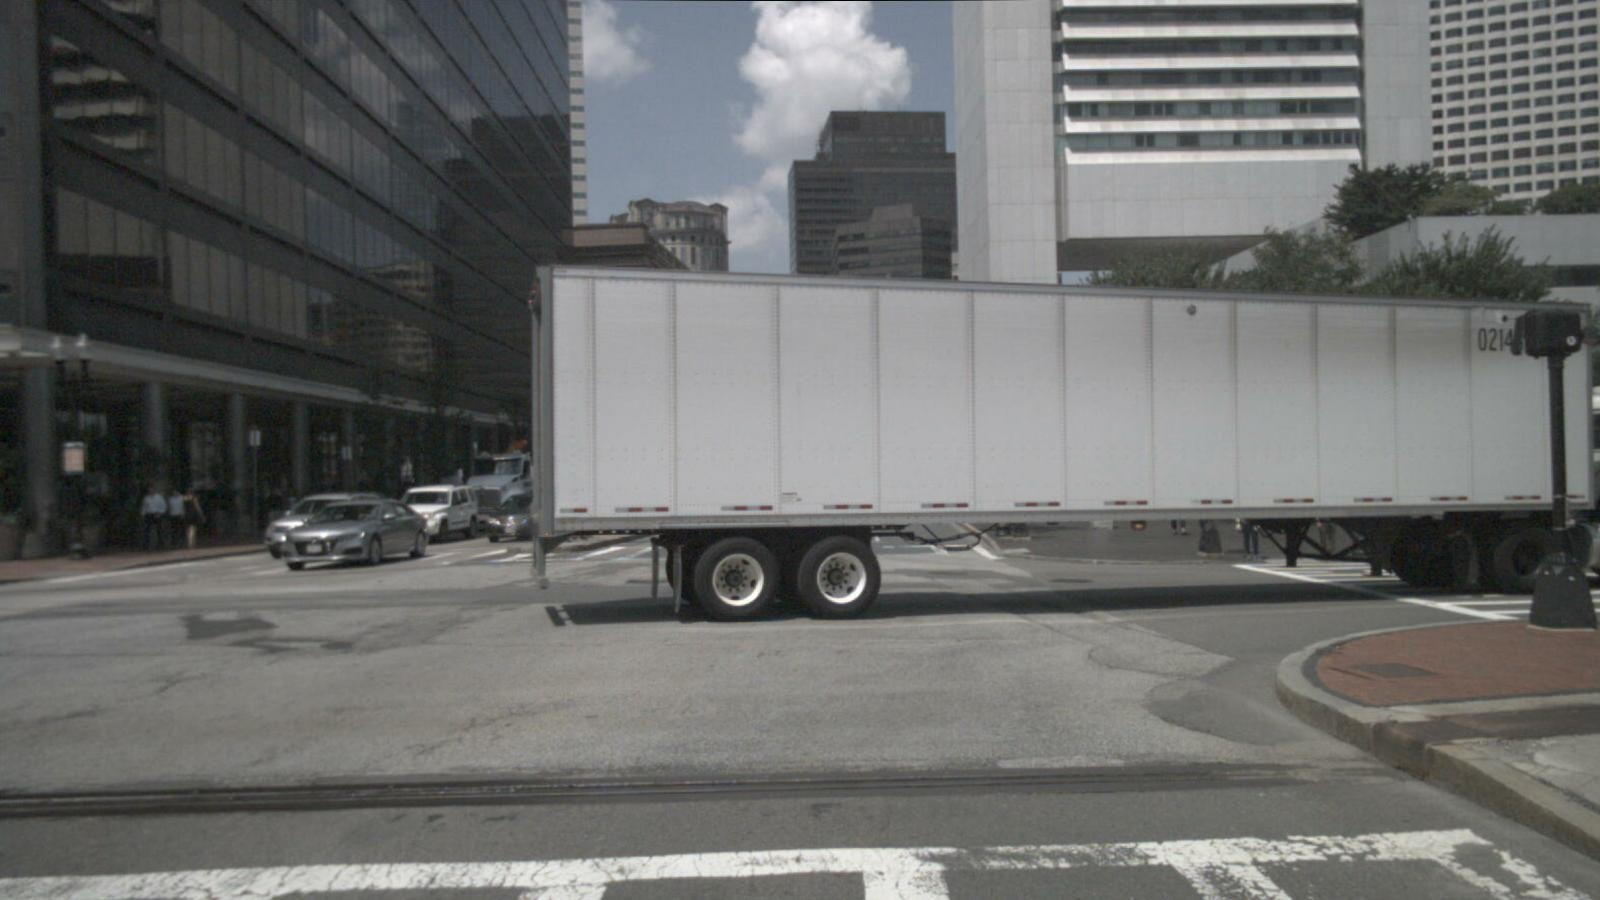
\includegraphics[width=12.8cm]{img/thumb_drivelm.jpg} &
    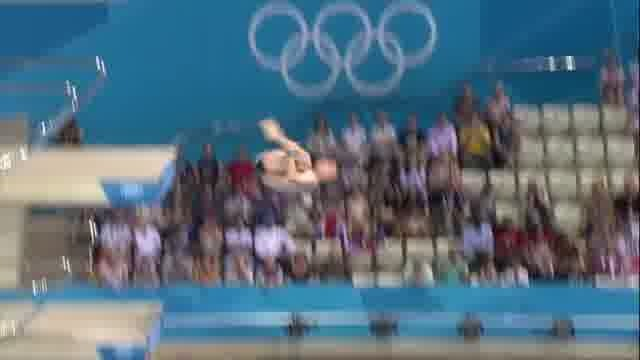
\includegraphics[width=12.8cm]{img/thumb_mtlaqa.jpg} \\[2mm]
    {\Large\textbf{DriveLM} · real} & {\Large\textbf{MTL-AQA} · real} \\[1mm]
    {\large\color{ink!70} 696 seq · avg 5.9 frames} & {\large\color{ink!70} 338 seq · avg 4.5 frames} \\
  \end{tabular}\\[9mm]
  \raggedright
  {\Large Near-identical consecutive frames are filtered out (LPIPS $<$ 0.05), so every swap is \textbf{perceptually visible} --- the anomaly is never hidden in lookalike frames.}
\end{minipage}
\hfill
\begin{minipage}[t]{0.62\linewidth}
  \beat{5}{What we ruled out}
  {\Large None of these explain the gap --- the limitation looks \textbf{structural, not incidental}.}\\[7mm]
  \centering
  \begin{tabular}{@{}c@{\hspace{12mm}}c@{}}
  % ---- (a) visual similarity -------------------------------------------
  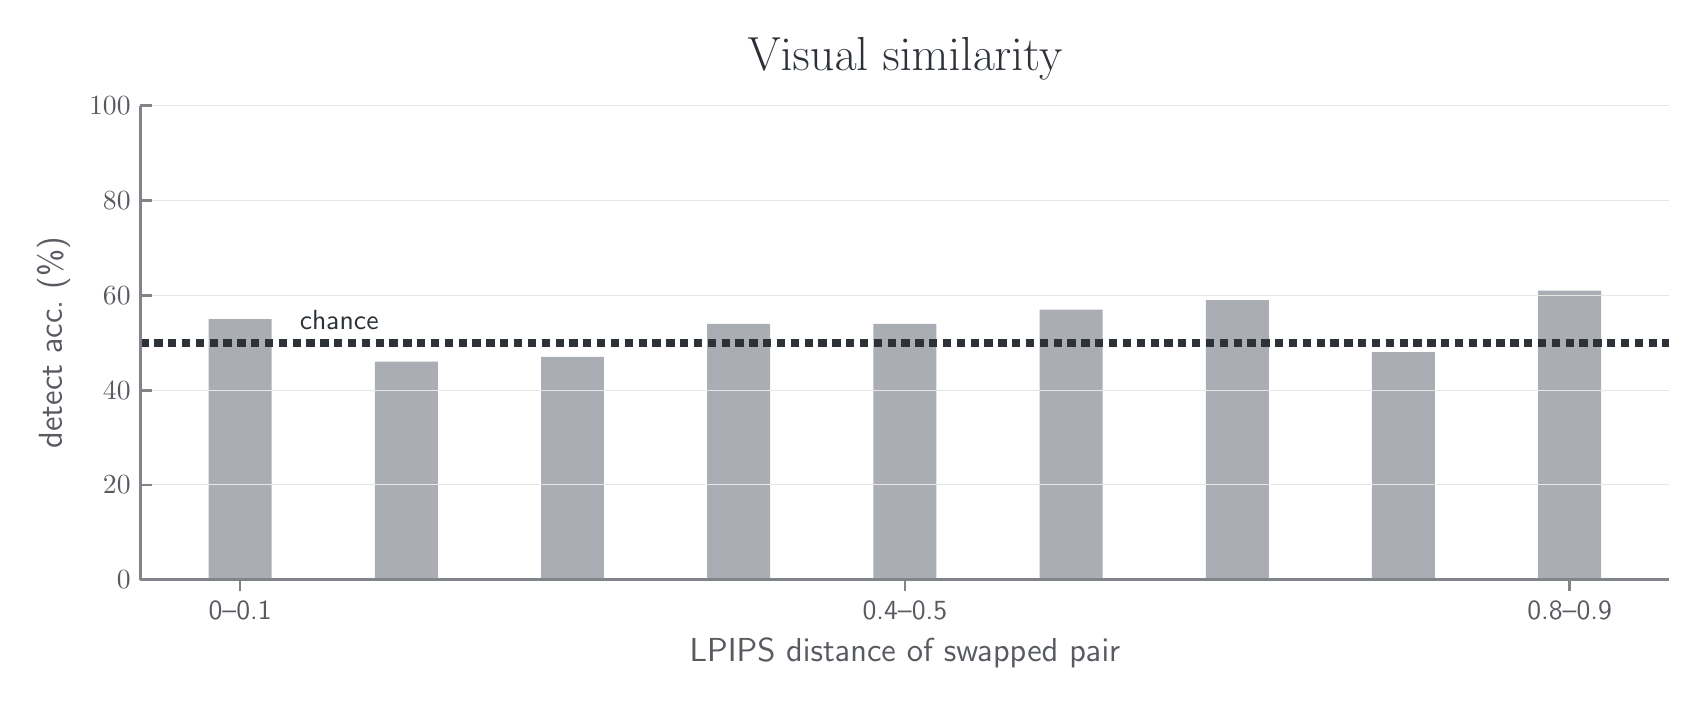
\begin{tikzpicture}
    \begin{axis}[mini, title={Visual similarity},
      ybar, bar width=8mm, ymin=0, ymax=100,
      xmin=0.4, xmax=9.6, xtick={1,5,9},
      xticklabels={0--0.1,0.4--0.5,0.8--0.9},
      xlabel={LPIPS distance of swapped pair}, ylabel={detect acc.\ (\%)}]
      \addplot[fill=neutral!55, draw=none] coordinates
        {(1,55)(2,46)(3,47)(4,54)(5,54)(6,57)(7,59)(8,48)(9,61)};
      \draw[densely dashed,ink,line width=1mm]
        (axis cs:0.4,50) -- (axis cs:9.6,50) node[pos=0.13,above,font=\normalsize]{chance};
    \end{axis}
  \end{tikzpicture} &
  % ---- (b) model scale --------------------------------------------------
  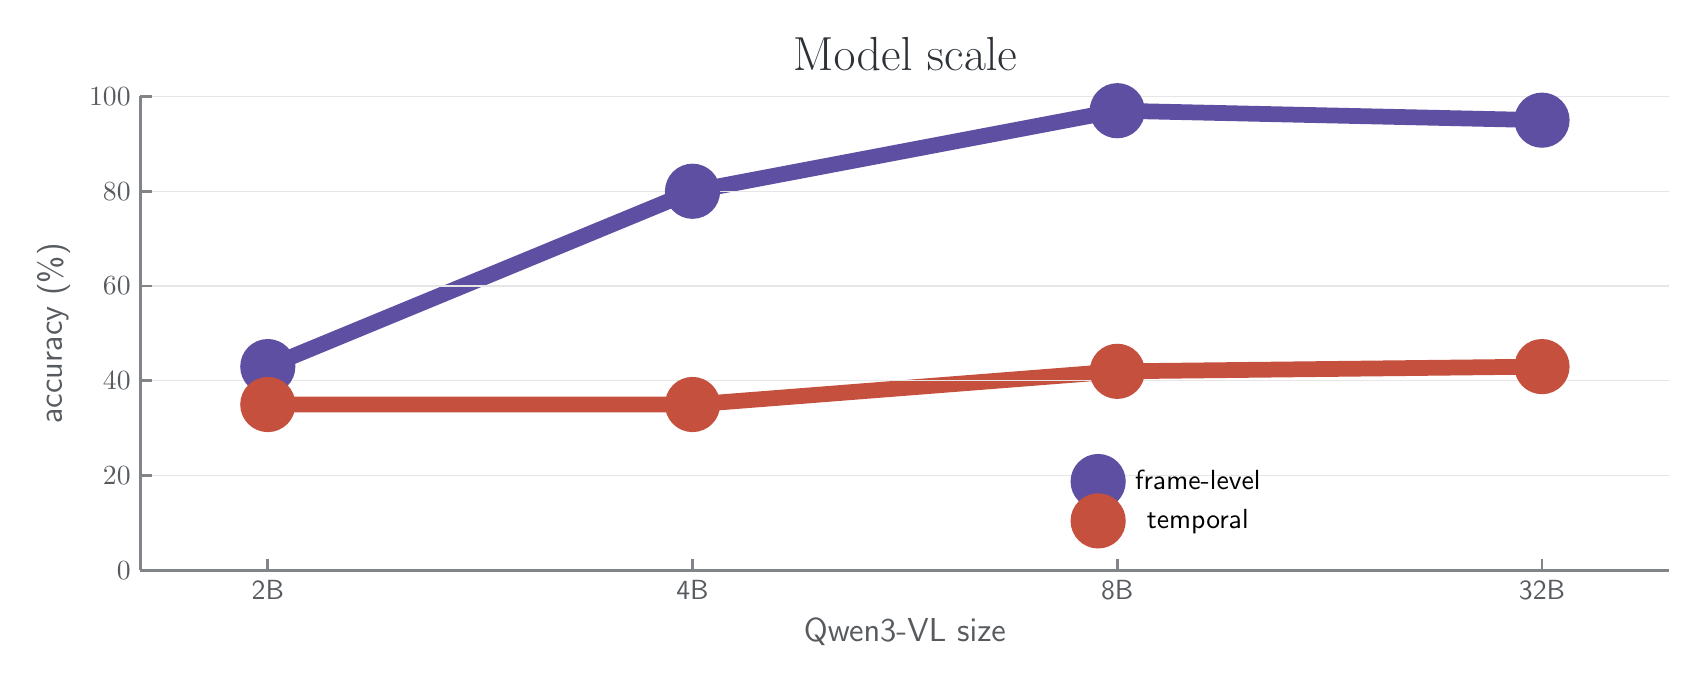
\begin{tikzpicture}
    \begin{axis}[mini, title={Model scale},
      ymin=0, ymax=100, xmin=0.7, xmax=4.3,
      xtick={1,2,3,4}, xticklabels={2B,4B,8B,32B},
      xlabel={Qwen3-VL size}, ylabel={accuracy (\%)},
      legend style={at={(0.6,0.05)}, anchor=south west}]
      \addplot[grape, line width=2mm, mark=*, mark size=2.5mm]
        coordinates {(1,43)(2,80)(3,97)(4,95)};
      \addplot[coral, line width=2mm, mark=*, mark size=2.5mm]
        coordinates {(1,35)(2,35)(3,42)(4,43)};
      \legend{frame-level, temporal}
    \end{axis}
  \end{tikzpicture} \\[3mm]
  {\Large\itshape near chance in every bin} & {\Large\itshape frame-level soars, temporal crawls} \\[9mm]
  % ---- (c) prompting -----------------------------------------------------
  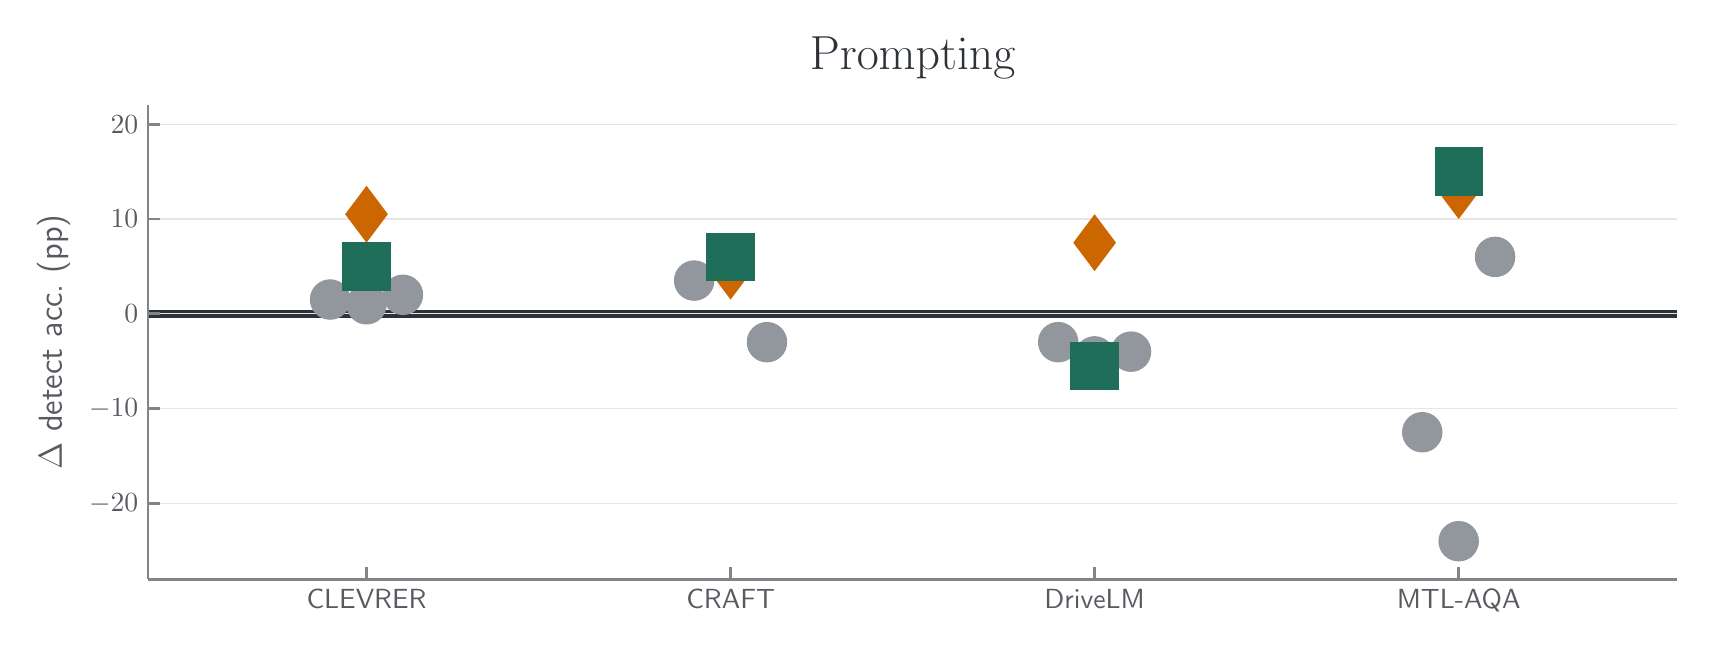
\begin{tikzpicture}
    \begin{axis}[mini, title={Prompting},
      ymin=-28, ymax=22, xmin=0.4, xmax=4.6,
      xtick={1,2,3,4}, xticklabels={CLEVRER,CRAFT,DriveLM,MTL-AQA},
      ylabel={$\Delta$ detect acc.\ (pp)}]
      \draw[ink,line width=1mm] (axis cs:0.4,0) -- (axis cs:4.6,0);
      \addplot[only marks, mark=*, mark size=2.5mm, neutral!70] coordinates
        {(0.9,1.5)(1,1)(1.1,2)(1.9,3.5)(2.1,-3)(2.9,-3)(3,-4.5)(3.1,-4)(3.9,-12.5)(4,-24)(4.1,6)};
      \addplot[only marks, mark=diamond*, mark size=3.5mm, orange!80!black] coordinates
        {(1,10.5)(2,4.5)(3,7.5)(4,13)};
      \addplot[only marks, mark=square*, mark size=3mm, hookteal] coordinates
        {(1,5)(2,6)(3,-5.5)(4,15)};
    \end{axis}
  \end{tikzpicture} &
  % ---- (d) sequence length ----------------------------------------------
  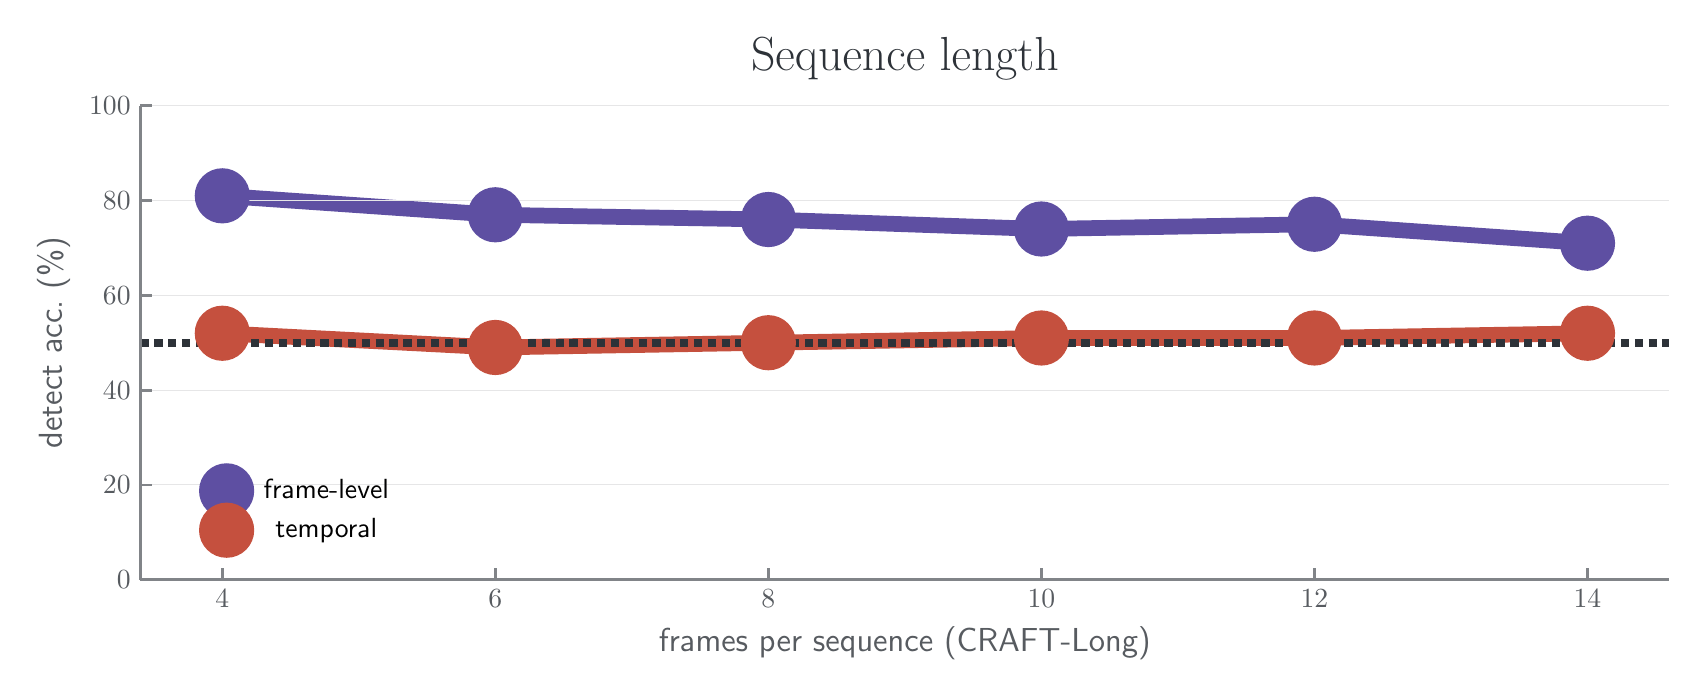
\begin{tikzpicture}
    \begin{axis}[mini, title={Sequence length},
      ymin=0, ymax=100, xmin=3.4, xmax=14.6,
      xtick={4,6,8,10,12,14},
      xlabel={frames per sequence (CRAFT-Long)}, ylabel={detect acc.\ (\%)},
      legend style={at={(0.03,0.05)}, anchor=south west}]
      \addplot[grape, line width=2mm, mark=*, mark size=2.5mm]
        coordinates {(4,81)(6,77)(8,76)(10,74)(12,75)(14,71)};
      \addplot[coral, line width=2mm, mark=*, mark size=2.5mm]
        coordinates {(4,52)(6,49)(8,50)(10,51)(12,51)(14,52)};
      \draw[densely dashed,ink,line width=1mm]
        (axis cs:3.4,50) -- (axis cs:14.6,50);
      \legend{frame-level, temporal}
    \end{axis}
  \end{tikzpicture} \\[3mm]
  \begin{tabular}{@{}c@{}}
    {\Large\itshape no consistent gain from any prompt}\\[1mm]
    {\normalsize \textcolor{neutral}{$\bullet$ prompt variants\quad}\textcolor{orange!80!black}{$\blacklozenge$ no scene text\quad}\textcolor{hookteal}{$\blacksquare$ thinking}}
  \end{tabular} & {\Large\itshape more frames don't help} \\
  \end{tabular}
\end{minipage}

\vspace{9mm}
\enlargethispage{25mm}

% ================================================================ BEAT 6 — TAKEAWAY
\beat{6}{Takeaway}
{\LARGE Current VLMs reason well about \textbf{individual frames} but not about how frames \textbf{relate over time}. TimeCatch isolates this by changing \emph{only} frame order --- everything else about the sequence stays the same. Scaling models up or changing prompts does not close the gap.}\\[4mm]
\raggedleft{\normalsize\color{ink!50} TimeCatch · Anonymous ACL submission · code and data to be released}

\end{document}
